\documentclass{article}

\usepackage{latexsym, amssymb}
\usepackage{graphicx}
\usepackage{rail}
\railoptions{-t -h}

\relax

\begin{document}

\title{Faust Quick Reference}
\author{Yann Orlarey\\Grame, Centre National de Creation Musicale}
\date{October 2007}


\railalias{recur}{$\sim$}
\railalias{lbrace}{\{}
\railalias{rbrace}{\}}
\railalias{dollar}{\$}
\railalias{mod}{\%}
\railalias{ampersand}{\&}
\railalias{hat}{$\land$}
\railalias{pipe}{$|$}
\railalias{fdelay}{}
\railalias{backslash}{\char"5C}
\railterm{recur,lbrace,rbrace,dollar,mod,ampersand,backslash,fdelay, pipe, hat}

\newcommand{\farg}[1]{\textrm{\textit{#1}}}
\newcommand{\ldbrack}{[\![ \,}
\newcommand{\rdbrack}{\, ]\!] }
\newcommand{\rdbrackC}{\rdbrack_{\mathrm{C}}\,}
\newcommand{\dbrack}[1]{\ldbrack #1 \rdbrack}
\newcommand{\semantic}[1]{\ldbrack #1 \rdbrack}
\newcommand{\dbrackC}[1]{\ldbrack #1 \rdbrackC}

\setlength{\parindent}{0pt}
\setlength{\parskip}{1ex plus 0.5ex minus 0.2ex}

\maketitle

\section{Introduction}

This document is a quick-reference to the Faust language (version 0.9.9.2), a programming language for real-time signal processing and synthesis that targets high-performance signal processing applications and audio plug-ins.

\section{Faust program}


A Faust program describes a \emph{signal processor} that transforms input signals into output signals. A Faust program is made of one or more source files. A source file is essentially a list of \emph{definitions} with the possibility to recursively import definitions from other source files. Each definition associates an identifier (with an optional list of parameters or an optional list of patterns) with a \emph{block-diagram} that it represents.

\begin{rail}
program : (definition | fileimport | declaration)+;
\end{rail}

\subsection{Definitions}
Faust is based on a declarative style of programming. A valid Faust program must contain at least one definition for the keyword \emph{process}  (the equivalent of \emph{main} in C) . Definitions can appear in any order. In particular an identifier can be used before being defined. Multiple definitions of the same identifier are treated as pattern-matching rules and analyzed as such.

\begin{rail}
definition  : "process" '=' blockdiagram ';'
			| ident (  | '(' (pattern + ',') ')' ) '=' blockdiagram ';';
pattern : ident | blockdiagram;
\end{rail}

% \begin{rail}
% parameterlist : '(' (identifier + ',') ')' ;
% \end{rail}
%

%  \begin{rail}
%  identifier : letter + (letter | digit );
%  letter : "a--zA--Z";
%  digit : "0--9";
%  \end{rail}

For example: 

\texttt{
\begin{tabular}{ll}
process &= +;\\
\end{tabular}
} 

is a valid Faust program that add its two input signals to produce its output. Here is a more involved example of \emph{noise} generetor:

\texttt{
\begin{tabular}{ll}
random 	&= +(12345) $\sim$ *(1103515245);\\
noise	&= random/2147483647.0;\\
process &= noise * vslider("vol", 0, 0, 1, 0.1);\\
\end{tabular}
}
 
\subsection{File Imports}

File imports allow to add the definitions of another source file to the definitions of the current file. File imports can appear every where in a source file and in any order. Mutual recursive imports are allowed and handled correctly.

\begin{rail}
fileimport : "import" '(' filename ')' ';';
\end{rail}

It is common for a Faust program to import the definitions of math.lib and music.lib files by including the lines : $\mathtt{import("math.lib");}$ and  $\mathtt{import("music.lib");}$.


\subsection{Declarations}

Declarations can be used to define some meta-data documenting and describing the project. The currently implemented meta-data are the name, the author, the version, the copyright and the license of the project. This information is typically used when generating an XML description of the project (option -xml of the compiler).

\begin{rail}
declaration : "declare" property string ';';
property : "name" | "author" | "copyright" | "license" | "version";
\end{rail}

Here is an example of declarations :

\begin{tabular}{l}
	\texttt{declare name "superFX";}\\
	\texttt{declare author "Alonzo Church";}\\
	\texttt{declare version "0.9.5c";}\\
\end{tabular}

\section{Block-Diagrams}

Faust is a \emph{block-diagram} language. Specific \emph{composition operations} are used to "connect" two block-diagrams together in order to form a new one.  For example the sequential composition operation (':') connect the outputs of the first block-diagram to the corresponding inputs of the second block-diagram. Five high-level composition operations are provided : \emph{recursive composition}, \emph{parallel composition}, \emph{sequential composition}, \emph{split composition} and \emph{merge composition}. Moreover a block-diagram can have an associated set of local definitions.

\vspace{5 mm}

\begin{tabular}{|l|l|l|}
\hline
\textbf{Syntax} & \textbf{Pri.}  & \textbf{Description} \\
\hline
\texttt{\farg{blockdiagram}\ $\sim$\ \farg{blockdiagram}}		& 4 & recursive composition     \\
\texttt{\farg{blockdiagram}\ ,\ \farg{blockdiagram}}			& 3 & parallel composition      \\
\texttt{\farg{blockdiagram}\ :\ \farg{blockdiagram}}			& 2 & sequential composition    \\
\texttt{\farg{blockdiagram}\ <:\ \farg{blockdiagram}}			& 1 & split composition      	\\
\texttt{\farg{blockdiagram}\ :>\ \farg{blockdiagram}}			& 1 & merge composition      	\\
\texttt{\farg{blockdiagram}\ with\ \{ \farg{definition} \dots \} }	& 0 & local definitions     \\
\texttt{\farg{expression}}										&  & block-diagrams are			\\
																&  & made of expressions    	\\
\hline
\end{tabular}

\vspace{5 mm}

All these composition operations are left associative. Based on these associativity and priority rules the block-diagram : $\mathtt{A:B,C\sim D,E :> F}$ should be interpreted as: $\mathtt{(A:((B,(C\sim D)),E)) :> F}$.


%%%%%%%%%%%%%%%%%%%%%%%%%%%%%%%%%%%%%%%%%%%%%%%%%%%%%%%%%%%%%%%%%%%%%%%%%%%%%%%%%%%%%%
%                            EXPRESSIONS                                             %
%%%%%%%%%%%%%%%%%%%%%%%%%%%%%%%%%%%%%%%%%%%%%%%%%%%%%%%%%%%%%%%%%%%%%%%%%%%%%%%%%%%%%%

\section{Expressions}

Faust \emph{Expressions} provide \emph{syntactic sugar} allowing traditional infix notation and function calls.
For example instead of : $\mathtt{2,A:*,B:+}$ one can write the infix expression : $\mathtt{2*A+B}$.
Or instead of : $\mathtt{A:\sin}$ one can use the function call notation : $\mathtt{\sin(A)}$.

\vspace{5 mm}

\begin{tabular}{|l|l|l|}
\hline
\textbf{Syntax} & \textbf{Pri.}  & \textbf{Description} \\
\hline
\texttt{\farg{expression}(\farg{arg},\ldots)}		& 10 & function call      \\
\texttt{\farg{expression}.\farg{ident}}				& 10 & access to lexical environment  \\

\texttt{\farg{expression}'}							& 9 & one sample delay \\
\texttt{\farg{expression} @ \farg{expression}} 		& 8 & fixed delay \\

\texttt{\farg{expression} * \farg{expression}} 		& 7 & multiplication \\
\texttt{\farg{expression} / \farg{expression}} 		& 7 & division	\\
\texttt{\farg{expression} \% \farg{expression}} 	& 7 & modulo \\
\texttt{\farg{expression} \& \farg{expression}} 	& 7 & logical and \\
\texttt{\farg{expression} $\land$ \farg{expression}} 	& 7 & logical xor \\
\texttt{\farg{expression} << \farg{expression}} 	& 7 & arithmetic left shift \\
\texttt{\farg{expression} >> \farg{expression}} 	& 7 & arithmetic right shift \\

\texttt{\farg{expression} + \farg{expression}}		& 6 & addition \\
\texttt{\farg{expression} - \farg{expression}} 		& 6 & substraction \\
\texttt{\farg{expression} | \farg{expression}} 		& 6 & logical or \\

\texttt{\farg{expression} <  \farg{expression}}		& 5 & less than \\
\texttt{\farg{expression} <= \farg{expression}} 	& 5 & less or equal \\
\texttt{\farg{expression} >  \farg{expression}}  	& 5 & greater than \\
\texttt{\farg{expression} >= \farg{expression}} 	& 5 & greater or equal \\
\texttt{\farg{expression} == \farg{expression}} 	& 5 & equal \\
\texttt{\farg{expression} != \farg{expression}}		& 5 & not equal \\

\texttt{\farg{primitive}} 							&   & expressions are made of primitives\\

\hline
\end{tabular}

\vspace{5 mm}

Binary operators can also be used in function call notation.
For example $\mathtt{+(2,A)}$ is equivalent to $\mathtt{2+A}$.
Moreover partial applications are allowed like in $\mathtt{*(3)}$.



%%%%%%%%%%%%%%%%%%%%%%%%%%%%%%%%%%%%%%%%%%%%%%%%%%%%%%%%%%%%%%%%%%%%%%%%%%%%%%%%%%%%%%
%                            PRIMITIVES                                             %
%%%%%%%%%%%%%%%%%%%%%%%%%%%%%%%%%%%%%%%%%%%%%%%%%%%%%%%%%%%%%%%%%%%%%%%%%%%%%%%%%%%%%%


\section{Primitive Signal Processing Operations}
The primitive signal processing operations represent the built-in functionalities of Faust, that is the atomic operations provided by the language.
All these primitives (and the block-diagrams build on top of them) denote \emph{signal processors}, functions transforming \emph{input signals} into \emph{output signals}.
Let's define more precisely what a \emph{signal processor} is.

A \emph{signal} $s$ is a discrete function of time
$s:\mathbb{N}\rightarrow\mathbb{R}$. The value of signal $s$ at time $t$
is written $s(t)$. We denote by $\mathbb{S}$ the set of all possible  signals :
$\mathbb{S}=\mathbb{N}\rightarrow\mathbb{R}$.
%
A \emph{n}-tuple of signals is written
$(s_{1},\ldots,s_{n})\in \mathbb{S}^{n}$.
The \emph{empty tuple}, single element of $\mathbb{S}^{0}$ is notated  $()$.
%
A \emph{signal processors} $p$ is a function from
\emph{n}-tuples of signals to \emph{m}-tuples of signals
$p:\mathbb{S}^{n}\rightarrow\mathbb{S}^{m}$. We notate $\mathbb{P}$ the
set of all signal processors :
$\mathbb{P}=\bigcup_{n,m}\mathbb{S}^{n}\rightarrow\mathbb{S}^{m}$.

All primitives and block-diagram expressed in Faust are members of $\mathbb{P}$ (i.e. signal processors) including numbers.
For example number 3.14 doesn't represent neither a sample, nor a signal, but a \emph{signal processor} : $\mathbb{S}^{0}\rightarrow\mathbb{S}^{1}$ that transforms the empty tuple $()$ into a 1-tuple of signals $(s)$ such that $\forall t\in\mathbb{N}, s(t)=3.14$.

%--------------------------------------------------------------------------------------------------------------
\subsection{C-equivalent primitives}
%--------------------------------------------------------------------------------------------------------------

Most Faust primitives are analogue to their C counterpart but lifted to signal processing.
For example $+$ is a function of type $\mathbb{S}^{2}\rightarrow\mathbb{S}^{1}$ that transforms a pair of signals $(x_1,x_2)$ into a 1-tuple of signals $(y)$ such that $\forall t\in\mathbb{N}, y(t)=x_{1}(t)+x_{2}(t)$.

\vspace{5 mm}

\begin{tabular}{|l|l|l|}
\hline
\textbf{Syntax} & \textbf{Type}  & \textbf{Description} \\
\hline
$n$ & $\mathbb{S}^{0}\rightarrow\mathbb{S}^{1}$ & integer number: $y(t)=n$ \\
$n.m$ & $\mathbb{S}^{0}\rightarrow\mathbb{S}^{1}$ & floating point number: $y(t)=n.m$ \\

\texttt{\_} & $\mathbb{S}^{1}\rightarrow\mathbb{S}^{1}$ & identity function: $y(t)=x(t)$ \\
\texttt{!} & $\mathbb{S}^{1}\rightarrow\mathbb{S}^{0}$ & cut function: $\forall x\in\mathbb{S},(x)\rightarrow ()$\\

\texttt{int} & $\mathbb{S}^{1}\rightarrow\mathbb{S}^{1}$ & cast into an int signal: $y(t)=(int)x(t)$  \\
\texttt{float} & $\mathbb{S}^{1}\rightarrow\mathbb{S}^{1}$ & cast into an float signal: $y(t)=(float)x(t)$  \\

\texttt{+} & $\mathbb{S}^{2}\rightarrow\mathbb{S}^{1}$ & addition: $y(t)=x_{1}(t)+x_{2}(t)$  \\
\texttt{-} & $\mathbb{S}^{2}\rightarrow\mathbb{S}^{1}$ & subtraction: $y(t)=x_{1}(t)-x_{2}(t)$   \\
\texttt{*} & $\mathbb{S}^{2}\rightarrow\mathbb{S}^{1}$ & multiplication: $y(t)=x_{1}(t)*x_{2}(t)$   \\
\texttt{/} & $\mathbb{S}^{2}\rightarrow\mathbb{S}^{1}$ & division: $y(t)=x_{1}(t)/x_{2}(t)$   \\
\texttt{\%} & $\mathbb{S}^{2}\rightarrow\mathbb{S}^{1}$ & modulo: $y(t)=x_{1}(t)\%x_{2}(t)$   \\

\texttt{\&} & $\mathbb{S}^{2}\rightarrow\mathbb{S}^{1}$ & logical AND: $y(t)=x_{1}(t)\&x_{2}(t)$   \\
\texttt{|} & $\mathbb{S}^{2}\rightarrow\mathbb{S}^{1}$ & logical OR: $y(t)=x_{1}(t)|x_{2}(t)$   \\
\texttt{$\land$} & $\mathbb{S}^{2}\rightarrow\mathbb{S}^{1}$ & logical XOR: $y(t)=x_{1}(t)\land x_{2}(t)$   \\

\texttt{<<} & $\mathbb{S}^{2}\rightarrow\mathbb{S}^{1}$ & arith. shift left: $y(t)=x_{1}(t) << x_{2}(t)$   \\
\texttt{>>} & $\mathbb{S}^{2}\rightarrow\mathbb{S}^{1}$ & arith. shift right: $y(t)=x_{1}(t) >> x_{2}(t)$   \\


\texttt{<} & $\mathbb{S}^{2}\rightarrow\mathbb{S}^{1}$ & less than: $y(t)=x_{1}(t) < x_{2}(t)$   \\
\texttt{<=} & $\mathbb{S}^{2}\rightarrow\mathbb{S}^{1}$ & less or equal: $y(t)=x_{1}(t) <= x_{2}(t)$   \\
\texttt{>} & $\mathbb{S}^{2}\rightarrow\mathbb{S}^{1}$ & greater than: $y(t)=x_{1}(t) > x_{2}(t)$   \\
\texttt{>=} & $\mathbb{S}^{2}\rightarrow\mathbb{S}^{1}$ & greater or equal: $y(t)=x_{1}(t) >= x_{2}(t)$   \\
\texttt{==} & $\mathbb{S}^{2}\rightarrow\mathbb{S}^{1}$ & equal: $y(t)=x_{1}(t) == x_{2}(t)$   \\
\texttt{!=} & $\mathbb{S}^{2}\rightarrow\mathbb{S}^{1}$ & different: $y(t)=x_{1}(t) != x_{2}(t)$   \\

\hline

\end{tabular}

\vspace{5 mm}


%--------------------------------------------------------------------------------------------------------------
\subsection{\texttt{math.h}-equivalent primitives}
%--------------------------------------------------------------------------------------------------------------

Most of the C \texttt{math.h} functions are also built-in as primitives (the others are defined as external functions in file \texttt{math.lib}).

\vspace{5 mm}
\begin{tabular}{|l|l|l|}
\hline
\textbf{Syntax} & \textbf{Type}  & \textbf{Description} \\
\hline

\texttt{acos} & $\mathbb{S}^{1}\rightarrow\mathbb{S}^{1}$ & arc cosine: $y(t)=\mathrm{acosf}(x(t))$ \\
\texttt{asin} & $\mathbb{S}^{1}\rightarrow\mathbb{S}^{1}$ & arc sine: $y(t)=\mathrm{asinf}(x(t))$ \\
\texttt{atan} & $\mathbb{S}^{1}\rightarrow\mathbb{S}^{1}$ & arc tangent: $y(t)=\mathrm{atanf}(x(t))$ \\
\texttt{atan2} & $\mathbb{S}^{2}\rightarrow\mathbb{S}^{1}$ & arc tangent of 2 signals: $y(t)=\mathrm{atan2f}(x_{1}(t), x_{2}(t))$ \\

\texttt{cos} & $\mathbb{S}^{1}\rightarrow\mathbb{S}^{1}$ & cosine: $y(t)=\mathrm{cosf}(x(t))$ \\
\texttt{sin} & $\mathbb{S}^{1}\rightarrow\mathbb{S}^{1}$ & sine: $y(t)=\mathrm{sinf}(x(t))$ \\
\texttt{tan} & $\mathbb{S}^{1}\rightarrow\mathbb{S}^{1}$ & tangent: $y(t)=\mathrm{tanf}(x(t))$ \\

\texttt{exp} & $\mathbb{S}^{1}\rightarrow\mathbb{S}^{1}$ & base-e exponential: $y(t)=\mathrm{expf}(x(t))$ \\
\texttt{log} & $\mathbb{S}^{1}\rightarrow\mathbb{S}^{1}$ & base-e logarithm: $y(t)=\mathrm{logf}(x(t))$ \\
\texttt{log10} & $\mathbb{S}^{1}\rightarrow\mathbb{S}^{1}$ & base-10 logarithm: $y(t)=\mathrm{log10f}(x(t))$ \\
\texttt{pow} & $\mathbb{S}^{2}\rightarrow\mathbb{S}^{1}$ & power: $y(t)=\mathrm{powf}(x_{1}(t),x_{2}(t))$ \\
\texttt{sqrt} & $\mathbb{S}^{1}\rightarrow\mathbb{S}^{1}$ & square root: $y(t)=\mathrm{sqrtf}(x(t))$ \\
\texttt{abs} & $\mathbb{S}^{1}\rightarrow\mathbb{S}^{1}$ & absolute value (int): $y(t)=\mathrm{abs}(x(t))$ \\
			&											 & absolute value (float): $y(t)=\mathrm{fabsf}(x(t))$ \\
\texttt{min} & $\mathbb{S}^{2}\rightarrow\mathbb{S}^{1}$ & minimum: $y(t)=\mathrm{min}(x_{1}(t),x_{2}(t))$ \\
\texttt{max} & $\mathbb{S}^{2}\rightarrow\mathbb{S}^{1}$ & maximum: $y(t)=\mathrm{max}(x_{1}(t),x_{2}(t))$ \\
\texttt{fmod} & $\mathbb{S}^{2}\rightarrow\mathbb{S}^{1}$ & float modulo: $y(t)=\mathrm{fmodf}(x_{1}(t),x_{2}(t))$ \\
\texttt{remainder} & $\mathbb{S}^{2}\rightarrow\mathbb{S}^{1}$ & float remainder: $y(t)=\mathrm{remainderf}(x_{1}(t),x_{2}(t))$ \\

\texttt{floor} & $\mathbb{S}^{1}\rightarrow\mathbb{S}^{1}$ & largest int $\leq$: $y(t)=\mathrm{floorf}(x(t))$ \\
\texttt{ceil} & $\mathbb{S}^{1}\rightarrow\mathbb{S}^{1}$ & smallest int $\geq$: $y(t)=\mathrm{ceilf}(x(t))$ \\
\texttt{rint} & $\mathbb{S}^{1}\rightarrow\mathbb{S}^{1}$ & closest int: $y(t)=\mathrm{rintf}(x(t))$ \\

\hline
\end{tabular}
\vspace{5 mm}





%--------------------------------------------------------------------------------------------------------------
\subsection{Delay, Table, Selector primitives}
%--------------------------------------------------------------------------------------------------------------

The following primitives allow to define fixed delays, read-only and read-write tables and 2 or 3-ways selectors (see figure \ref{fig:delays}).

\vspace{5 mm}
\begin{tabular}{|l|l|l|}
\hline
\textbf{Syntax} & \textbf{Type}  & \textbf{Description} \\
\hline

\texttt{mem} & $\mathbb{S}^{1}\rightarrow\mathbb{S}^{1}$ 		& 1-sample delay: 	$y(t+1)=x(t),y(0)=0$  \\
\texttt{prefix} & $\mathbb{S}^{2}\rightarrow\mathbb{S}^{1}$ 	& 1-sample delay:  	$y(t+1)=x_{2}(t),y(0)=x_{1}(0)$  \\
\texttt{@} & $\mathbb{S}^{2}\rightarrow\mathbb{S}^{1}$ 			& fixed delay:  	$y(t+x_{2}(t))=x_{1}(t), y(t<x_{2}(t))=0$  \\

\texttt{rdtable} & $\mathbb{S}^{3}\rightarrow\mathbb{S}^{1}$ 	& read-only table:	$y(t)=T[r(t)]$  \\
\texttt{rwtable} & $\mathbb{S}^{5}\rightarrow\mathbb{S}^{1}$ 	& read-write table:	$T[w(t)]=c(t); y(t)=T[r(t)]$  \\

\texttt{select2} & $\mathbb{S}^{3}\rightarrow\mathbb{S}^{1}$ 	& select between 2 signals:	$T[]=\{x_{0}(t),x_{1}(t)\}; y(t)=T[s(t)]$  \\
\texttt{select3} & $\mathbb{S}^{4}\rightarrow\mathbb{S}^{1}$ 	& select between 3 signals:	$T[]=\{x_{0}(t),x_{1}(t),x_{2}(t)\}; y(t)=T[s(t)]$  \\

\hline
\end{tabular}
\vspace{5 mm}


\begin{figure}
\centering
\includegraphics[scale=0.6]{illustrations/faust-diagram4}
\includegraphics[scale=0.6]{illustrations/faust-diagram5}
\includegraphics[scale=0.6]{illustrations/faust-diagram6}
\caption{Delays, tables and selectors primitives }
\label{fig:delays}
\end{figure}


%--------------------------------------------------------------------------------------------------------------
\subsection{User Interface Elements}
%--------------------------------------------------------------------------------------------------------------


Faust user interface widgets allow an abstract description of the user interface from within the Faust code. This description is
independent of any GUI toolkits. It is based on \emph{buttons}, \emph{checkboxes}, \emph{sliders}, etc. that are grouped together vertically and
horizontally using appropriate grouping schemes.

All these GUI elements produce signals. A button for example (see figure \ref{fig:button}) produces a signal which is 1 when the button is pressed and 0 otherwise.
These signals can be freely combined with other audio signals.

\begin{figure}[h]
\centering
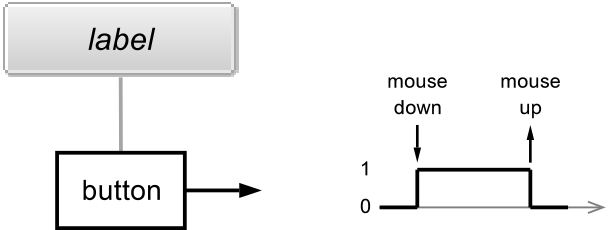
\includegraphics[scale=0.5]{illustrations/button}
\caption{User Interface Button}
\label{fig:button}
\end{figure}


\vspace{5 mm}

\begin{tabular}{|l|l|}
\hline
\textbf{Syntax} & \textbf{Example} \\
\hline
\texttt{button(\farg{str})} & \texttt{button("play")}\\
\texttt{checkbox(\farg{str})} & \texttt{checkbox("mute")}\\
\texttt{vslider(\farg{str},\farg{cur},\farg{min},\farg{max},\farg{step})} & \texttt{vslider("vol",50,0,100,1)}\\
\texttt{hslider(\farg{str},\farg{cur},\farg{min},\farg{max},\farg{step})} & \texttt{hslider("vol",0.5,0,1,0.01)}\\
\texttt{nentry(\farg{str},\farg{cur},\farg{min},\farg{max},\farg{step})} & \texttt{nentry("freq",440,0,8000,1)}\\
\texttt{vgroup(\farg{str},\farg{block-diagram})} & \texttt{vgroup("reverb", \ldots)}\\
\texttt{hgroup(\farg{str},\farg{block-diagram})} & \texttt{hgroup("mixer", \ldots)}\\
\texttt{tgroup(\farg{str},\farg{block-diagram})} & \texttt{vgroup("parametric", \ldots)}\\
\texttt{vbargraph(\farg{str},\farg{min},\farg{max})} & \texttt{vbargraph("input",0,100)}\\
\texttt{hbargraph(\farg{str},\farg{min},\farg{max})} & \texttt{hbargraph("signal",0,1.0)}\\
\hline
\end{tabular}

\vspace{5 mm}

\textbf{note} : The \emph{str} string used in widgets can contain variable parts.
These variable parts are indicated by the sign '\texttt{\%}' followed by the name of a variable.
For example \texttt{par(i,8,hslider("Voice \%i", 0.9, 0, 1, 0.01))} creates 8 different sliders in parallel :
\texttt{hslider("Voice 0", 0.9, 0, 1, 0.01),}
\texttt{hslider("Voice 1", 0.9, 0, 1, 0.01),} \ldots
\texttt{,hslider("Voice 7", 0.9, 0, 1, 0.01)}.

An escape mechanism is provided.
If the sign '\texttt{\%}' is followed by itself, it will be included in the resulting string.
For example \texttt{"feedback (\%\%)"} will result in \texttt{"feedback (\%)"}.



%--------------------------------------------------------------------------------------------------------------
\subsection{Foreign Functions and Constants}
%--------------------------------------------------------------------------------------------------------------

Any C function or constant can be introduced using the foreign function mechanism.
It allows to declare an external C function by indicating its name and signature as well as the required include file.
The syntax of foreign function and foreign constant declarations is the following :

\begin{rail}
foreign : 'ffunction' '(' signature ',' includefile ',' comment ')' | 'fconstant' '(' type identifier ',' includefile ')' ;
signature : type identifier '(' (type * ',') ')';
type : 'int' | 'float';
\end{rail}


The file \texttt{math.lib} included in the Faust package defines most of the standard mathematical function of
\texttt{<math.h>} (that are not already builtins) using the foreign function mechanism.
Here is the list of these functions :

\vspace{5 mm}

\begin{tabular}{|l|l|}
\hline
\textbf{Name} & \textbf{Definition}   \\
\hline

\texttt{SR 			} & \texttt{ fconstant(int fSamplingFreq, <math.h>)} \\
\texttt{PI 			} & \texttt{ 3.1415926535897932385 } \\
\texttt{cbrt 		} & \texttt{ ffunction(float cbrt (float), <math.h>,"")} \\
\texttt{hypot 		} & \texttt{ ffunction(float hypot (float, float), <math.h>,"")} \\
\texttt{ldexp 		} & \texttt{ ffunction(float ldexp (float, int), <math.h>,"")} \\
\texttt{scalb 		} & \texttt{ ffunction(float scalb (float, float), <math.h>,"")} \\
\texttt{log1p 		} & \texttt{ ffunction(float log1p (float), <math.h>,"")} \\
\texttt{logb 		} & \texttt{ ffunction(float logb (float), <math.h>,"")} \\
\texttt{ilogb 		} & \texttt{ ffunction(int ilogb (float), <math.h>,"")} \\
\texttt{expm1 		} & \texttt{ ffunction(float expm1 (float), <math.h>,"")} \\
\texttt{acosh		} & \texttt{ ffunction(float acosh (float), <math.h>, "")} \\
\texttt{asinh		} & \texttt{ ffunction(float asinh (float), <math.h>, "")} \\
\texttt{atanh		} & \texttt{ ffunction(float atanh (float), <math.h>, "")} \\
\texttt{sinh		} & \texttt{ ffunction(float sinh (float), <math.h>, "")} \\
\texttt{cosh		} & \texttt{ ffunction(float cosh (float), <math.h>, "")} \\
\texttt{tanh		} & \texttt{ ffunction(float tanh (float), <math.h>,"")} \\
\texttt{erf			} & \texttt{ ffunction(float erf(float), <math.h>,"")} \\
\texttt{erfc		} & \texttt{ ffunction(float erfc(float), <math.h>,"")} \\
\texttt{gamma		} & \texttt{ ffunction(float gamma(float), <math.h>,"")} \\
\texttt{J0			} & \texttt{ ffunction(float j0(float), <math.h>,"")} \\
\texttt{J1			} & \texttt{ ffunction(float j1(float), <math.h>,"")} \\
\texttt{Jn			} & \texttt{ ffunction(float jn(int, float), <math.h>,"")} \\
\texttt{lgamma		} & \texttt{ ffunction(float lgamma(float), <math.h>,"")} \\
\texttt{Y0			} & \texttt{ ffunction(float y0(float), <math.h>,"")} \\
\texttt{Y1			} & \texttt{ ffunction(float y1(float), <math.h>,"")} \\
\texttt{Yn			} & \texttt{ ffunction(float yn(int, float), <math.h>,"")} \\
\texttt{isnan 		} & \texttt{ ffunction(int isnan (float),<math.h>,"")} \\
\texttt{nextafter	} & \texttt{ ffunction(float nextafter(float, float),<math.h>,"")} \\
\hline
\end{tabular}

\vspace{5 mm}

%--------------------------------------------------------------------------------------------------------------
\subsection{Programming constructions}
%--------------------------------------------------------------------------------------------------------------

Faust provides several programming constructions that give powerful ways to describe and transform block-diagrams algorithmically.

\begin{rail}
Abstraction :  backslash '(' (ident + ',') ')' '.' '(' blockdiagram ')';
\end{rail} 
\emph{Abstractions} allow to define anonymous functions like for example a square function : $\char"5C (x).(x*x)$. Unapplied abstractions can be used for symbolic routing of signals. For example : $\char"5C (x,y).(y,x)$ denotes a signal processor that exchanges its two inputs. 

\begin{rail}
Case :  "case" lbrace (rule +) rbrace ;
Rule : '(' (pattern + ',') ')' "=>" blockdiagram ';';
Pattern : ident | blockdiagram;
\end{rail}
\emph{case} pattern matching rules provide an effective way to analyze and transform block-diagrams algorithmically. For example \texttt{case\{ (x:y) => y:x; (x) => x; \}} will invert the two parts of a sequential block-diagram and leave untouched any other construction. Please note that patterns are evaluated before the pattern matching operation. Thefore only variables that appear free in the pattern are binding variables during pattern matching. 


\begin{rail}
Component : 'component' '(' filename ')';
\end{rail}
The \emph{component} construction allows a very modular design. A whole Faust program can be included in another Faust program as a simple expression. For example \texttt{component("freeverb.dsp")} denotes the process defined in the file \emph{"freeverb.dsp"}, and 

\begin{tabular}{l}
\texttt{process = component("karplus32.dsp"):component("freeverb.dsp");} \\
\end{tabular}

is a process that combines two components in sequence.

\begin{rail}
par : "par" '(' ident ',' value ',' blockdiagram ')';
seq : "seq" '(' ident ',' value ',' blockdiagram ')';
sum : "sum" '(' ident ',' value ',' blockdiagram ')';
prod : "prod" '(' ident ',' value ',' blockdiagram ')';
\end{rail}
The \texttt{par}, \texttt{seq}, \texttt{sum} and \texttt{prod} constructions allow algorithmic descriptions of block-diagrams.
For example :

\begin{tabular}{lll}
\texttt{par(i,8,E(i))} &is equivalent to &\texttt{E(0),E(1),\ldots ,E(7)} \\
\texttt{seq(i,8,E(i))} &is equivalent to &\texttt{E(0):E(1):\ldots :E(7)} \\
\texttt{sum(i,8,E(i))} &is equivalent to &\texttt{E(0)+E(1)+\ldots +E(7)} \\
\texttt{prod(i,8,E(i))} &is equivalent to &\texttt{E(0)*E(1)*\ldots *E(7)}\\
\end{tabular}


%%%%%%%%%%%%%%%%%%%%%%%%%%%%%%%%%%%%%%%%%%%%%%%%%%%%%%%%%%%%%%%%%%%%%%%%%%%%%%%%%%%%%%
%                            INVOKING THE COMPILER                                             %
%%%%%%%%%%%%%%%%%%%%%%%%%%%%%%%%%%%%%%%%%%%%%%%%%%%%%%%%%%%%%%%%%%%%%%%%%%%%%%%%%%%%%%


\section{Invoking the Faust compiler}
The Faust compiler is invoked using the \texttt{faust} command. It translate Faust programs into C++ code.
The generated code can be wrapped into an optional \emph{architecture file} allowing to directly produce a fully operational program.

\begin{rail}
compiler : "faust" (|options) ( file +);
\end{rail}


Compilation options are listed in the following table :

\vspace{5 mm}

\begin{tabular}{|l|l|l|}
\hline
\textbf{Short} 				& \textbf{long} 					& \textbf{Description}   \\
\hline
\texttt{-h} 				& \texttt{--help} 					& print the help message  \\
\texttt{-v} 				& \texttt{--version} 				& print version information  \\
\texttt{-d} 				& \texttt{--details} 				& print compilation details  \\
\texttt{-ps} 				& \texttt{--postscript} 			& generate block-diagram postscript file  \\
\texttt{-svg} 				& \texttt{--svg} 					& generate block-diagram svg files  \\
\texttt{-f \farg{n}} 		& \texttt{--fold \farg{n}}  		& max complexity of svg diagrams before splitting\\
							&									& into several files (default 25 boxes)  \\
\texttt{-mns \farg{n}} 		& \texttt{--max-name-size \farg{n}} & max character size used in svg diagram labels\\
							&									& (default max size : 40 chars) \\
\texttt{-xml} 				& \texttt{--xml} 					& generate an additional description file in xml format  \\
\texttt{-lb}	 			& \texttt{--left-balanced} 			& generate left-balanced expressions  \\
\texttt{-mb} 				& \texttt{--mid-balanced} 			& generate mid-balanced expressions (default)  \\
\texttt{-rb} 				& \texttt{--right-balanced}			& generate right-balanced expressions  \\
\texttt{-a \farg{file}} 	&  									& C++ wrapper file  \\
\texttt{-o \farg{file}} 	&  									& C++ output file  \\
\hline
\end{tabular}

\vspace{5 mm}

The main available architecture files are :

\vspace{5 mm}

\begin{tabular}{|l|l|l|}
\hline
\textbf{File name}			& \textbf{Description}   \\
\hline
\texttt{max-msp.cpp} 		& Max/MSP plugin  \\
\texttt{vst.cpp} 			& VST plugin  \\
\texttt{jack-gtk.cpp} 		& Jack GTK full application  \\
\texttt{jack-qt.cpp} 		& Jack QT full application  \\
\texttt{alsa-gtk.cpp} 		& Alsa GTK full application  \\
\texttt{alsa-qt.cpp} 		& Alsa QT full application  \\
\texttt{oss-gtk.cpp} 		& OSS GTK full application  \\
\texttt{ladspa.cpp} 		& LADSPA plugin  \\
\texttt{q.cpp} 				& Q language plugin  \\
\texttt{supercollider.cpp} 	& SuperCollider Unit Generator  \\
\texttt{sndfile.cpp} 		& sound file transformation command \\
\texttt{bench.cpp} 			& speed benchmark   \\

\hline
\end{tabular}

\vspace{5 mm}

Here is an example of compilation command that generates the C++ source code of a Jack application using the GTK graphic toolkit:

\texttt{faust -a jack-gtk.cpp -o freeverb.cpp freeverb.dsp}.

\vspace{5 mm}

%%%%%%%%%%%%%%%%%%%%%%%%%%%%%%%%%%%%%%%%%%%%%%%%%%%%%%%%%%%%%%%%%%%%%%%%%%%%%%%%%%%%%%
%%%%%%%%%%%%%%%%%%%%%%%%%%%%%%%%%%%%%%%%%%%%%%%%%%%%%%%%%%%%%%%%%%%%%%%%%%%%%%%%%%%%%%
%                            		END                                              %
%%%%%%%%%%%%%%%%%%%%%%%%%%%%%%%%%%%%%%%%%%%%%%%%%%%%%%%%%%%%%%%%%%%%%%%%%%%%%%%%%%%%%%
%%%%%%%%%%%%%%%%%%%%%%%%%%%%%%%%%%%%%%%%%%%%%%%%%%%%%%%%%%%%%%%%%%%%%%%%%%%%%%%%%%%%%%


\end{document}
